\documentclass[11pt,a4paper]{article}

% -----------------------------------------------------------------------------
% Encoding & Typography (using pre-installed TeX Live packages)
% -----------------------------------------------------------------------------
\usepackage[utf8]{inputenc}
\usepackage{lmodern}
\usepackage[T1]{fontenc}
\usepackage[scaled=0.92]{lato}
\usepackage{graphicx}
\usepackage{xcolor}
\usepackage{tikz}
\usetikzlibrary{shapes.geometric, arrows.meta, positioning, calc, fit, backgrounds}
\usepackage{tcolorbox}
\usepackage{enumitem}
\usepackage{array}
\usepackage{tabularx}
\usepackage{colortbl}
\usepackage{placeins}
\usepackage{url}
\usepackage{hyperref}

% -----------------------------------------------------------------------------
% Page Geometry (A4: 210mm x 297mm, ~25mm margins)
% -----------------------------------------------------------------------------
\setlength{\paperwidth}{210mm}
\setlength{\paperheight}{297mm}
\setlength{\textwidth}{160mm}
\setlength{\textheight}{238mm}
\setlength{\oddsidemargin}{0mm}
\setlength{\evensidemargin}{0mm}
\setlength{\topmargin}{-10mm}
\setlength{\headheight}{14pt}
\setlength{\headsep}{10mm}
\setlength{\footskip}{12mm}
\setlength{\parindent}{0pt}
\setlength{\parskip}{6pt}
\emergencystretch=2em

% -----------------------------------------------------------------------------
% Color Palette (Systems & Networking Technical Report)
% -----------------------------------------------------------------------------
\definecolor{chibablue}{RGB}{20, 65, 130}
\definecolor{chibateal}{RGB}{0, 120, 130}
\definecolor{chibadark}{RGB}{35, 40, 48}
\definecolor{codebg}{RGB}{246, 248, 250}
\definecolor{codeframe}{RGB}{208, 215, 222}
\definecolor{noteaccent}{RGB}{30, 100, 180}
\definecolor{notebg}{RGB}{240, 246, 255}
\definecolor{warnaccent}{RGB}{190, 90, 0}

% -----------------------------------------------------------------------------
% Hyperref Setup
% -----------------------------------------------------------------------------
\hypersetup{
    colorlinks=true,
    linkcolor=chibablue,
    urlcolor=chibateal,
    citecolor=chibablue,
    pdftitle={ClickHouse Ingestion and Behavioural Analysis (CHIBA) - Technical Report},
    pdfauthor={Giuseppe Nozza},
    pdfsubject={Network Telemetry and Behavioural Anomaly Detection}
}

% -----------------------------------------------------------------------------
% Running Headers & Footers
% -----------------------------------------------------------------------------
\makeatletter
\def\@oddhead{\small\sffamily\textcolor{gray}{CHIBA --- ClickHouse Ingestion and Behavioural Analysis}\hfill\textcolor{gray}{\leftmark}}
\def\@evenhead{\small\sffamily\textcolor{gray}{\leftmark}\hfill\textcolor{gray}{CHIBA Technical Report}}
\def\@oddfoot{\hfill\small\sffamily\textcolor{gray}{Page \thepage}\hfill}
\def\@evenfoot{\hfill\small\sffamily\textcolor{gray}{Page \thepage}\hfill}
\makeatother

% -----------------------------------------------------------------------------
% Custom Environments for Code Blocks & Callouts
% -----------------------------------------------------------------------------
\newenvironment{codebox}[1][]{%
    \begin{tcolorbox}[
        colback=codebg,
        colframe=codeframe,
        boxrule=0.6pt,
        arc=1.5mm,
        left=3mm,
        right=3mm,
        top=2mm,
        bottom=2mm,
        fonttitle=\sffamily\bfseries\footnotesize,
        coltitle=chibadark,
        colbacktitle=codeframe!50!white,
        #1
    ]
}{%
    \end{tcolorbox}
}

\newenvironment{notebox}[1][Note]{%
    \begin{tcolorbox}[
        colback=notebg,
        colframe=noteaccent,
        boxrule=0.7pt,
        arc=1.5mm,
        left=3.5mm,
        right=3.5mm,
        top=2.5mm,
        bottom=2.5mm,
        title={#1},
        fonttitle=\sffamily\bfseries\small
    ]
}{%
    \end{tcolorbox}
}

% List spacing
\setlist[itemize]{topsep=3pt, itemsep=3pt, parsep=2pt}
\setlist[enumerate]{topsep=3pt, itemsep=3pt, parsep=2pt}

% Graphics path
\graphicspath{{../img/}{img/}}

% -----------------------------------------------------------------------------
% Document Begin
% -----------------------------------------------------------------------------
\begin{document}

% -----------------------------------------------------------------------------
% Title Page
% -----------------------------------------------------------------------------
\begin{titlepage}
    \centering
    \vspace*{1.5cm}

    {\scshape\Large\sffamily\textcolor{chibateal}{Network Management --- Academic Year 2025/2026}\par}
    \vspace{0.8cm}
    {\color{chibablue}\rule{\textwidth}{1.5pt}\par}
    \vspace{0.6cm}
    {\huge\bfseries\sffamily\textcolor{chibadark}{ClickHouse Ingestion and Behavioural Analysis (CHIBA)}\par}
    \vspace{0.6cm}
    {\color{chibablue}\rule{\textwidth}{1.5pt}\par}

    \vspace{2cm}

    {\large\sffamily\textbf{Author:} Giuseppe Nozza\par}
    \vspace{0.25cm}
    {\normalsize\sffamily\textbf{Course Instructor:} \href{https://luca.ntop.org/}{Prof.\ Luca Deri}\par}
    \vspace{0.3cm}
    {\normalsize\sffamily\textcolor{gray}{\today}\par}

    \vfill
\end{titlepage}

% -----------------------------------------------------------------------------
% Table of Contents
% -----------------------------------------------------------------------------
\pagenumbering{roman}
\tableofcontents
\newpage
\pagenumbering{arabic}

% =============================================================================
% SECTION 1: PROJECT DESCRIPTION
% =============================================================================
\section{Project Description}

\subsection{Objectives}
The purpose of this telemetry tool is to analyze the behavior of network flows in real time and from PCAP files in order to detect Distributed Denial-of-Service (DDoS) attacks, data exfiltration, horizontal network scans, and both fast and slow vertical port scans.

\subsection{From Probe Capture to Binary Export}

Figure~\ref{fig:daemon_arch} illustrates the internal process and thread architecture of the CHIBA daemon, from initial bootstrap and packet capture to bulk binary ingestion into ClickHouse.

\begin{figure}[htbp]
\centering
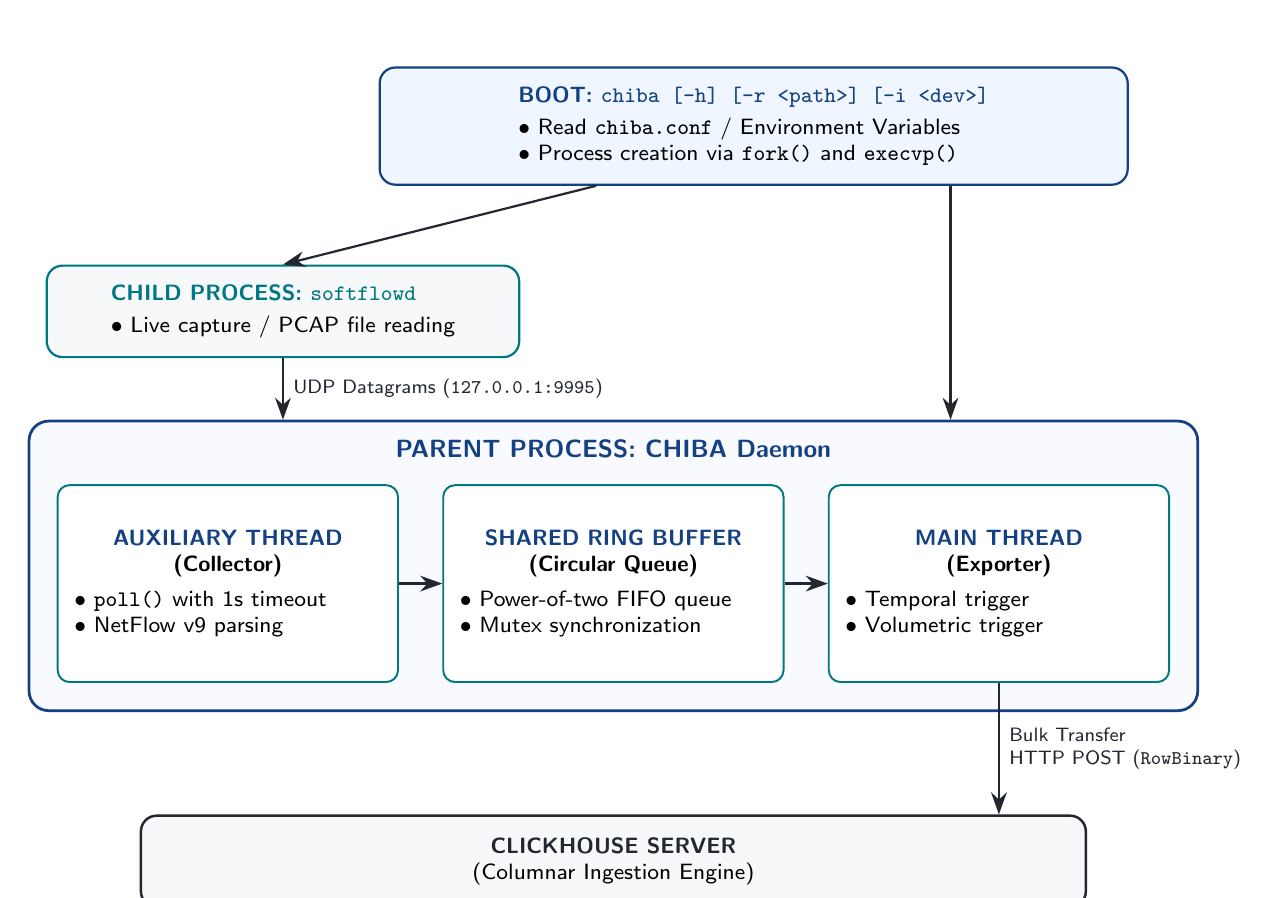
\begin{tikzpicture}[
    font=\sffamily\footnotesize,
    node distance=0.8cm and 0.6cm,
    box/.style={
        rectangle, rounded corners=2mm, draw=chibablue, line width=0.8pt,
        fill=notebg, align=left, inner sep=7pt
    },
    subbox/.style={
        rectangle, rounded corners=1.5mm, draw=chibateal, line width=0.7pt,
        fill=white, align=left, inner sep=6pt, minimum height=2.5cm, text width=3.9cm
    },
    dbbox/.style={
        rectangle, rounded corners=2mm, draw=chibadark, line width=0.9pt,
        fill=codebg, align=center, inner sep=8pt, minimum width=12cm
    },
    arrow/.style={-{Stealth[length=2.8mm, width=2mm]}, line width=0.8pt, draw=chibadark}
]

% Boot Node
\node[box, minimum width=9.5cm] (boot) {
    \textbf{\textcolor{chibablue}{BOOT: \texttt{chiba [-h] [-r <path>] [-i <dev>]}}}\\[2pt]
    $\bullet$ Read \texttt{chiba.conf} / Environment Variables\\
    $\bullet$ Process creation via \texttt{fork()} and \texttt{execvp()}
};

% Child Process Node
\node[box, below left=1.0cm and -1.8cm of boot, minimum width=6.0cm, fill=codebg, draw=chibateal] (child) {
    \textbf{\textcolor{chibateal}{CHILD PROCESS: \texttt{softflowd}}}\\[2pt]
    $\bullet$ Live capture / PCAP file reading
};

% Parent Daemon Subcomponents
\node[subbox, below=1.6cm of child, xshift=-0.7cm] (collector) {
    \centering\textbf{\textcolor{chibablue}{AUXILIARY THREAD}}\\
    \centering\textbf{(Collector)}\par\vspace{3pt}
    \raggedright
    $\bullet$ \texttt{poll()} with 1s timeout\\
    $\bullet$ NetFlow v9 parsing
};

\node[subbox, right=0.55cm of collector] (ringbuf) {
    \centering\textbf{\textcolor{chibablue}{SHARED RING BUFFER}}\\
    \centering\textbf{(Circular Queue)}\par\vspace{3pt}
    \raggedright
    $\bullet$ Power-of-two FIFO queue\\
    $\bullet$ Mutex synchronization
};

\node[subbox, right=0.55cm of ringbuf] (exporter) {
    \centering\textbf{\textcolor{chibablue}{MAIN THREAD}}\\
    \centering\textbf{(Exporter)}\par\vspace{3pt}
    \raggedright
    $\bullet$ Temporal trigger\\
    $\bullet$ Volumetric trigger
};

% Parent Daemon Container
\coordinate[above=0.45cm of ringbuf] (daemontop);
\begin{scope}[on background layer]
    \node[
        rectangle, rounded corners=2.5mm, draw=chibablue, line width=1pt,
        fill=notebg!50!white, inner sep=10pt,
        fit=(collector) (ringbuf) (exporter) (daemontop),
        label={[anchor=north, font=\sffamily\bfseries\small, text=chibablue, yshift=-4pt]north:PARENT PROCESS: CHIBA Daemon}
    ] (daemon) {};
\end{scope}

% ClickHouse Node
\node[dbbox, below=1.3cm of daemon] (clickhouse) {
    \textbf{\textcolor{chibadark}{CLICKHOUSE SERVER}}\\
    (Columnar Ingestion Engine)
};

% Connections
\draw[arrow] ([xshift=-2.0cm]boot.south) -- (child.north);
\draw[arrow] ([xshift=2.5cm]boot.south) -- ([xshift=2.5cm]boot.south |- daemon.north);
\draw[arrow] (child.south) -- node[right, font=\sffamily\scriptsize, text=chibadark] {UDP Datagrams (\texttt{127.0.0.1:9995})} (child.south |- daemon.north);
\draw[arrow] (collector.east) -- (ringbuf.west);
\draw[arrow] (ringbuf.east) -- (exporter.west);
\draw[arrow] (exporter.south) -- node[right, font=\sffamily\scriptsize, align=left, text=chibadark] {Bulk Transfer\\HTTP POST (\texttt{RowBinary})} (exporter.south |- clickhouse.north);

\end{tikzpicture}
\caption{End-to-end architecture of the CHIBA daemon and its interaction with \texttt{softflowd} and ClickHouse.}
\label{fig:daemon_arch}
\end{figure}

\subsubsection{CLI Parsing and Configuration Management}
Command-line interface (CLI) parsing is implemented using the POSIX \texttt{getopt()} function. The network traffic source is defined during this stage; live capture mode on a network interface and offline capture mode from a PCAP file are mutually exclusive.

The parameters required to build the URL for ClickHouse's HTTP ingestion interface are extracted from the \texttt{chiba.conf} configuration file via the \texttt{load\_config()} routine. These parameters can be overridden at runtime through dedicated environment variables. Below is the output produced when running \texttt{chiba} with the help flag (\texttt{-h}). Details regarding the execution path are covered in Section~2.

\begin{codebox}[title={CLI Help Output}]
\footnotesize
\begin{verbatim}
./bin/chiba -h
[INFO] chiba.conf read correctly.
Usage: chiba [-h] [-r <path>] [-i <device>]

Options:
  -h               Print help
  -r <path>        Static PCAP file path
  -i <device>      Live network interface name

Environment Variables for ClickHouse HTTP interface (override chiba.conf):
  CH_HOST          Host (default: 127.0.0.1)
  CH_DB            Database (default: chiba)
  CH_TABLE         Destination table (default: ingest_flows)
\end{verbatim}
\end{codebox}

\subsubsection{Managing \texttt{softflowd}}
The \texttt{softflowd} probe is instantiated by \texttt{chiba} via \texttt{fork()} and \texttt{execvp()}, running in the background as a concurrent child process while the parent process proceeds with daemon initialization.

The child process's \texttt{stdout} and \texttt{stderr} descriptors are redirected to \texttt{/dev/null} to prevent interference with CHIBA's logs.

NetFlow v9 records are exported to the collector thread via UDP datagrams (on \texttt{127.0.0.1:9995}). UDP is chosen for clear performance reasons, eliminating the connection, handshake, and acknowledgment overhead typical of TCP in favor of maximum throughput.

The argument array passed to \texttt{execvp()} differentiates capture parameters and flow export policies according to the operating mode:
\begin{itemize}
    \item \textbf{Live Mode:} The probe captures traffic in real time from the specified network interface. Flow timeouts are balanced for continuous monitoring: each flow has a maximum lifetime of 60 seconds before export; UDP inactivity timeout is set to a maximum of 30 seconds, while inactive TCP flows are exported within 5 minutes. This trade-off prevents saturation of \texttt{softflowd}'s active flow table and avoids excessive fragmentation of long-lived connections, ensuring up-to-date data reaches the collector without generating unnecessary network overhead.
    \item \textbf{Offline Mode:} The probe sequentially processes a static PCAP trace. Time constraints (maximum lifetime and emission intervals) are reduced to 1 second, and the flow table is constrained to its minimum size. This forces immediate eviction of every flow record toward the UDP socket, enabling rapid scanning of the packet dump without the pauses and idle intervals of the original traffic.
\end{itemize}

Immediately after \texttt{fork()}, the parent process performs a non-blocking check on the probe's status via:
\begin{codebox}[title={Non-Blocking Child Process Check (C)}]
\footnotesize
\begin{verbatim}
if (waitpid(pid, &status, WNOHANG) > 0) { ... }
\end{verbatim}
\end{codebox}
Using the \texttt{WNOHANG} flag avoids blocking and allows immediate detection of any startup failure in \texttt{softflowd} (for instance, due to a non-existent interface, insufficient privileges, or an invalid PCAP file path).

Finally, safe termination of the child process is handled by the daemon upon shutdown (or upon completion of PCAP file processing): CHIBA sends a \texttt{SIGTERM} signal to the recorded PID and invokes \texttt{waitpid()} in blocking mode to reap the process exit status, preventing zombie processes from lingering in the system.

\subsubsection{Parsing NetFlow v9 Records}
The responsibility of the collector thread is to receive the UDP packets sent by the probe and transform them into structured records ready for the database. Adopting NetFlow v9 entails additional complexity compared to rigid formats such as NetFlow v5: packets do not have a fixed structure, but instead decouple schema definitions from actual flow data.

At startup and at regular intervals, the probe transmits schema packets (\textbf{Template FlowSets}) that declare the composition of a flow: which fields are present, their sequence order, and their size in bytes. The parser stores these definitions in a static internal table for the entire duration of execution, without resorting to dynamic heap memory allocations.

When packets containing actual traffic (\textbf{Data FlowSets}) arrive, the parser consults the cached schema and extracts field values directly from the binary payload. Three primary operations are performed during this stage:
\begin{itemize}
    \item \textbf{Byte Decoding and Endianness Conversion:} Traffic counters and network ports are extracted according to their actual byte length (ranging from 1 to 8 bytes) and converted from network byte order (big-endian) to the host architecture's native byte order.
    \item \textbf{Address Space Unification:} To handle IPv4 and IPv6 simultaneously with a single unified logic, IPv4 addresses are mapped into the standard 128-bit \texttt{IPv4-mapped} IPv6 format (\texttt{::ffff:a.b.c.d}). This guarantees that every flow has an identical Layer-3 representation regardless of the underlying IP protocol version.
    \item \textbf{Normalization into Internal Format:} Extracted values are written into a compact structure derived from standard Cisco telemetry fields:
\end{itemize}

\begin{codebox}[title={Internal Flow Record Structure (\texttt{include/flow.h})}]
\footnotesize
\begin{verbatim}
typedef struct flow_data {
  u_int32_t start_time;
  u_int32_t end_time;

  u_int8_t  srcaddr[16];
  u_int8_t  dstaddr[16];

  u_int32_t dPkts;
  u_int32_t dOctets;
  u_int16_t srcport;
  u_int16_t dstport;
  u_int8_t  prot;
} __attribute__((packed)) flow_data;
\end{verbatim}
\end{codebox}

Using the \texttt{\_\_attribute\_\_((packed))} compiler attribute prevents the compiler from inserting padding bytes for structure alignment. Consequently, the structure has a net byte size that matches the exact binary sequence expected by ClickHouse for direct HTTP insertion, enabling bulk transfer of the entire memory block in \texttt{RowBinary} format without intermediate serialization steps.

\paragraph{NetFlow v9 Parsing Fixes and PCAP Trace Requirements}
\begin{itemize}
    \item \textbf{Complete FlowSet Scanning:} In the NetFlow v9 specification (RFC~3954), \texttt{header->count} indicates the total number of records (both template and data records) rather than the number of FlowSets. To prevent premature loop termination that previously caused templates and data records to be dropped in multi-FlowSet datagrams (such as in \texttt{DHCPv6.pcap}), packet scanning is driven by the total buffer length (\texttt{while (offset + sizeof(...) <= length)}).
    \item \textbf{Encapsulation Requirement for \texttt{softflowd} (\texttt{DLT\_NULL} Endianness):} On \texttt{x86\_64} architectures, \texttt{softflowd} requires packets to use standard Ethernet encapsulation (\texttt{DLT\_EN10MB}). In packet dumps captured on BSD loopback interfaces in big-endian order (\texttt{DLT\_NULL}, e.g., \texttt{snmp\_usm.pcap}), the 4-byte Address Family header is not byte-swapped by \texttt{libpcap}, causing \texttt{softflowd} to discard all traffic as \texttt{non-IP}. To allow \texttt{softflowd} to process such captures, they must be normalized to Ethernet using \texttt{tcprewrite -{}-dlt=enet}. Because the original capture lacks Ethernet frames, dummy source and destination MAC addresses must be supplied explicitly:
\begin{codebox}
\footnotesize
\begin{verbatim}
tcprewrite --dlt=enet \
  --enet-dmac=00:11:22:33:44:55 \
  --enet-smac=aa:bb:cc:dd:ee:ff \
  -i ./pcap/snmp_usm.pcap \
  -o ./pcap/snmp_usm_enet.pcap
\end{verbatim}
\end{codebox}
    \item \textbf{Temporal Alignment to Present Time:} In PCAP mode, CHIBA assigns the current system timestamp (\texttt{time(NULL)}) to ingested flows. This prevents the creation of historical partitions in ClickHouse and allows immediate visualization of plots within Grafana's default ``Today'' dashboards.
\end{itemize}

\subsubsection{Producer-Consumer Pattern and Double Buffering}
Decoupling high-frequency UDP packet reception from database persistence relies on the producer-consumer pattern, implemented through a shared circular queue (\texttt{ring\_buffer}). The auxiliary collector thread acts as the producer by inserting decoded flow records, while the main thread acts as the consumer by extracting accumulated records to send to ClickHouse.

Access to the shared resource is governed by a single \texttt{mutex}, deliberately omitting condition variables. Condition variables are unnecessary because the consumer does not need to wake up on every single insertion, nor does the producer wait for the queue to drain: the main thread evaluates extraction based on asymmetric triggers (either exceeding a volumetric threshold of accumulated records or reaching a maximum elapsed time interval). Eliminating calls to \texttt{pthread\_cond\_signal} and \texttt{pthread\_cond\_wait} removes context-switch overhead and minimizes lock holding time.

During bulk transfer invocations, memory management leverages a \emph{double buffering} strategy: while a batch of flows is isolated and transmitted over HTTP, the producer has the remaining free half of the ring buffer available to continue recording incoming flows, preventing packet drops or overwrites of unconsumed data in the queue.

\paragraph{Ring Buffer Implementation Notes}
The circular queue does not implement a traditional single-element extraction routine (\texttt{pop} element by element). Extraction occurs exclusively in contiguous blocks during bulk transfer, eliminating per-record synchronization overhead and minimizing contention on the shared mutex.

Advancing the circular indices leverages a buffer size strictly constrained to a power of two ($2^{15} = 32768$). This algebraic property makes it possible to compute wrapped indices without the modulo operator (\texttt{\%}), applying a fast bitwise AND mask instead:
\begin{codebox}[title={Bitwise Ring Buffer Index Advancement (C)}]
\footnotesize
\begin{verbatim}
/* Single-record enqueue (Producer) */
rb->tail = (rb->tail + 1) & (rb->size - 1);

/* Batch head advancement by n records (Consumer) */
rb->head = (rb->head + n) & (rb->size - 1);
\end{verbatim}
\end{codebox}

\subsubsection{HTTP Streaming}
The main thread manages flow transmission to ClickHouse by extracting accumulated records whenever the volumetric batch threshold (\texttt{EXPORT\_BUFFER\_SIZE = 16384}) is reached or the configured time interval (\texttt{EXPORT\_MIN\_TIME\_MS = 5000} ms) expires.

Data extracted from the circular queue first passes through a linear export buffer (\texttt{export\_buffer}). This intermediate staging buffer is necessary for two reasons: first, it linearizes memory whenever a batch of flows wraps around the physical boundary between the end and the beginning of the ring buffer; second, it allows the shared mutex to be released immediately after the memory copy operation, avoiding holding the lock during network I/O.

\paragraph{Flow Ingestion via \texttt{libcurl-easy}}
Adopting \texttt{libcurl}'s synchronous \texttt{easy} interface allows the exporter thread to manage the HTTP channel linearly across four sequential steps:
\begin{itemize}
    \item \textbf{Endpoint Configuration:} The request targets the local ClickHouse instance by passing the SQL \texttt{INSERT} statement directly as a URL query parameter specifying the \texttt{RowBinary} format. This keeps the SQL command definition separate from the \texttt{POST} request body, which is reserved entirely for the raw binary data stream.
    \item \textbf{Payload Binding:} The linear buffer is attached directly to the \texttt{POST} request body along with the total byte count to transmit. Because the \texttt{RowBinary} format contains no headers, metadata, or delimiter characters, ClickHouse interprets the stream by reading memory sequentially and mapping it positionally (1:1) onto the columns of the destination table. This design eliminates all computational overhead associated with text formatting or serialization.
    \item \textbf{Transfer Execution:} Transmission occurs synchronously via \texttt{curl\_easy\_perform()}, blocking the exporter thread until the batch upload completes. Furthermore, \texttt{libcurl}'s connection pool automatically reuses the underlying TCP connection across consecutive batches, reducing overall latency.
    \item \textbf{Response Validation:} Upon completion of the transfer, the HTTP response returned by the DBMS is inspected to verify that the current batch was persisted successfully before resetting buffer pointers and proceeding with the next accumulation cycle.
\end{itemize}

\subsubsection{Memory Cleanup}
All dynamic heap memory allocations and system resource acquisitions are strictly confined to the initial configuration and runtime setup phase. During this startup phase, the parent process validates CLI arguments, opens the UDP socket descriptor, spawns the child probe process, drops user privileges to \texttt{nobody}, allocates the ring and export buffers, initializes the \texttt{libcurl} context, and launches the auxiliary collector thread.

During the steady-state monitoring phase---after the auxiliary thread has been launched---no calls to \texttt{malloc()} or \texttt{free()} are ever executed.

Resource deallocation mirrors the acquisition sequence through a strict Last-In, First-Out (LIFO) cascade. When the daemon stops---triggered either by \texttt{SIGINT}/\texttt{SIGTERM} signal handlers or by child process termination at the end of a PCAP trace---the program exits its main loop and deallocates components in reverse order of allocation. Below is the cleanup sequence directly from \texttt{main.c}:

\begin{codebox}[title={Graceful LIFO Teardown (\texttt{src/main.c})}]
\footnotesize
\begin{verbatim}
/* LIFO cleanup */
curl_easy_cleanup(curl);
curl_global_cleanup();
export_buffer_destroy(eb);
ring_buffer_destroy(rb);

kill(pid, SIGTERM);
waitpid(pid, NULL, 0);
close(sockfd);

puts("[INFO] Shutting down");
return (EXIT_SUCCESS);
\end{verbatim}
\end{codebox}

If an initialization or allocation error occurs in any component during startup, resources acquired up to that point are unwound via an ordered chain of \texttt{goto} labels:

\begin{codebox}[title={Cascading Error Unwinding via \texttt{goto} (\texttt{src/main.c})}]
\footnotesize
\begin{verbatim}
/* LIFO cascade cleanup */
err_curl_easy:
    curl_easy_cleanup(curl);
err_curl_global:
    curl_global_cleanup();
err_eb:
    export_buffer_destroy(eb);
err_rb:
    ring_buffer_destroy(rb);
err_child:
    kill(pid, SIGTERM);
    waitpid(pid, NULL, 0);
err_socket:
    close(sockfd);

fprintf(stderr, "[ERROR] Shutting down: see error above\n");
return (EXIT_FAILURE);
\end{verbatim}
\end{codebox}

\paragraph{Valgrind Verification}
Memory management correctness and complete resource deallocation were verified using Valgrind by subjecting the daemon to two distinct operational scenarios with explicit tracking of heap blocks and file descriptors.

The first test verifies the full program lifecycle on a static PCAP trace containing IPv6 traffic:
\begin{codebox}[title={Valgrind Verification --- Offline PCAP Mode}]
\footnotesize
\begin{verbatim}
valgrind --leak-check=full --show-leak-kinds=all --track-fds=yes \
  ./bin/chiba -r ./pcap/DHCPv6.pcap

==16921== FILE DESCRIPTORS: 4 open (3 std) at exit.
==16921== Open AF_UNIX socket 12: <unknown>
==16921==    <inherited from parent>
==16921== 
==16921== HEAP SUMMARY:
==16921==     in use at exit: 0 bytes in 0 blocks
==16921==   total heap usage: 4,293 allocs, 4,293 frees, 2,842,787 bytes allocated
==16921== 
==16921== All heap blocks were freed -- no leaks are possible
==16921== 
==16921== ERROR SUMMARY: 0 errors from 0 contexts (suppressed: 0 from 0)
\end{verbatim}
\end{codebox}
The report confirms a 1:1 match between allocations and frees. File descriptor analysis confirms proper closure of the receiving UDP socket and redirected pipes; the single non-standard open descriptor is inherited from the parent shell process, ruling out any resource leak inside the daemon.

The second test verifies that the program also passes all memory and descriptor checks when interrupted asynchronously via a signal during live capture:
\begin{codebox}[title={Valgrind Verification --- Live Capture Mode with Asynchronous Interrupt}]
\footnotesize
\begin{verbatim}
valgrind --leak-check=full --show-leak-kinds=all --track-fds=yes ./bin/chiba -i lo

==17519==
==17519== FILE DESCRIPTORS: 3 open (3 std) at exit.
==17519==
==17519== HEAP SUMMARY:
==17519==     in use at exit: 0 bytes in 0 blocks
==17519==   total heap usage: 4,315 allocs, 4,315 frees, 2,858,557 bytes allocated
==17519==
==17519== All heap blocks were freed -- no leaks are possible
==17519==
==17519== For lists of detected and suppressed errors, rerun with: -s
==17519== ERROR SUMMARY: 0 errors from 0 contexts (suppressed: 0 from 0)
\end{verbatim}
\end{codebox}

\FloatBarrier
\newpage
\subsection{ClickHouse Schema and Data Pipeline}

Figure~\ref{fig:ch_pipeline} illustrates the multi-stage ClickHouse storage and analytical pipeline, from raw binary flow ingestion to pre-aggregated state tables, logical merge views, and Grafana visualization.

\begin{figure}[!ht]
\centering
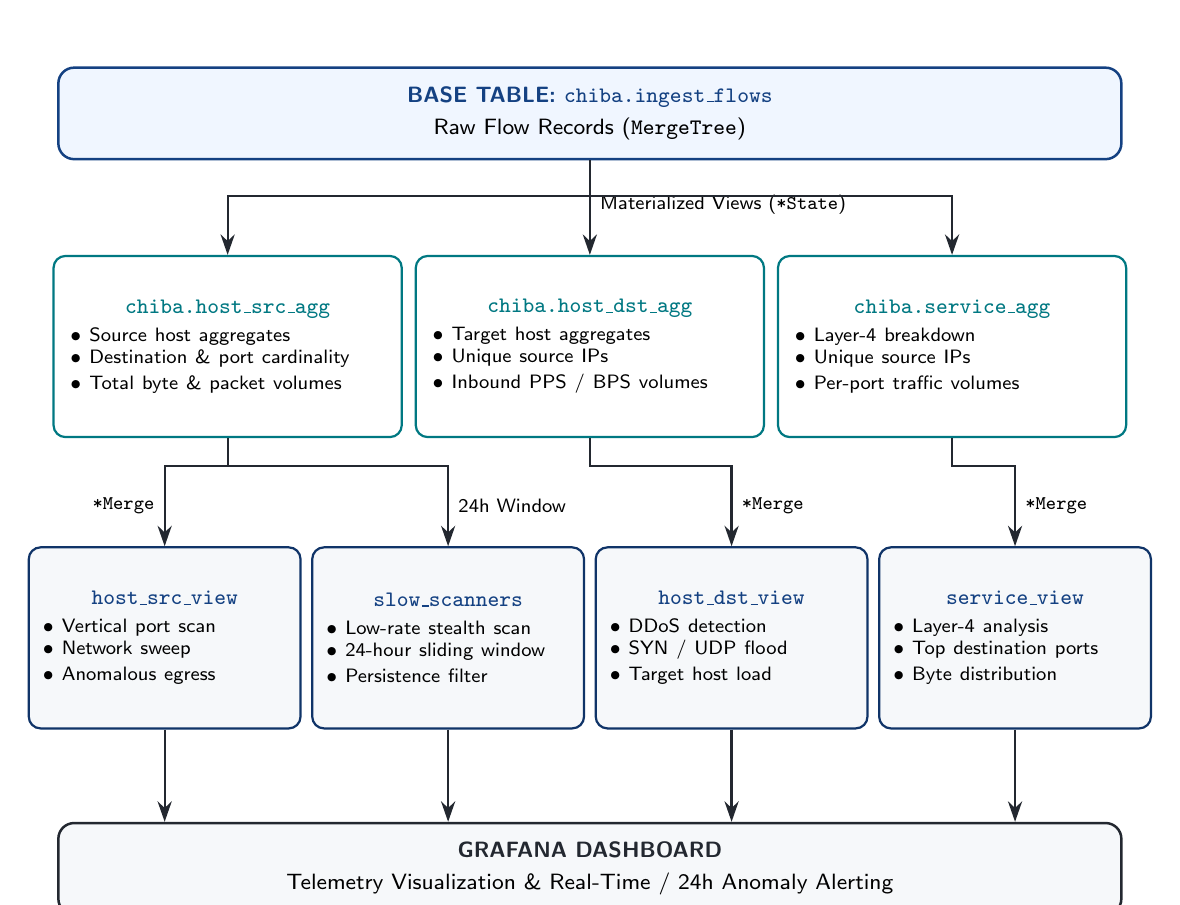
\begin{tikzpicture}[
    font=\sffamily\footnotesize,
    basebox/.style={
        rectangle, rounded corners=2mm, draw=chibablue, line width=0.9pt,
        fill=notebg, align=center, inner sep=7pt, minimum width=13.5cm
    },
    aggbox/.style={
        rectangle, rounded corners=1.5mm, draw=chibateal, line width=0.8pt,
        fill=white, align=left, inner sep=6pt, text width=4.0cm, minimum height=2.3cm
    },
    viewbox/.style={
        rectangle, rounded corners=1.5mm, draw=chibablue!80!black, line width=0.8pt,
        fill=codebg, align=left, inner sep=5pt, text width=3.1cm, minimum height=2.3cm
    },
    arrow/.style={-{Stealth[length=2.6mm, width=1.8mm]}, line width=0.8pt, draw=chibadark}
]

% Base Table
\node[basebox] (ingest) {
    \textbf{\textcolor{chibablue}{BASE TABLE: \texttt{chiba.ingest\_flows}}}\\[2pt]
    Raw Flow Records (\texttt{MergeTree})
};

% Aggregating Tables
\node[aggbox, below=1.2cm of ingest, xshift=-4.6cm] (srcagg) {
    \centering\textbf{\textcolor{chibateal}{\texttt{chiba.host\_src\_agg}}}\par\vspace{2pt}
    \raggedright\scriptsize
    $\bullet$ Source host aggregates\\
    $\bullet$ Destination \& port cardinality\\
    $\bullet$ Total byte \& packet volumes
};

\node[aggbox, below=1.2cm of ingest] (dstagg) {
    \centering\textbf{\textcolor{chibateal}{\texttt{chiba.host\_dst\_agg}}}\par\vspace{2pt}
    \raggedright\scriptsize
    $\bullet$ Target host aggregates\\
    $\bullet$ Unique source IPs\\
    $\bullet$ Inbound PPS / BPS volumes
};

\node[aggbox, below=1.2cm of ingest, xshift=4.6cm] (srvagg) {
    \centering\textbf{\textcolor{chibateal}{\texttt{chiba.service\_agg}}}\par\vspace{2pt}
    \raggedright\scriptsize
    $\bullet$ Layer-4 breakdown\\
    $\bullet$ Unique source IPs\\
    $\bullet$ Per-port traffic volumes
};

% Logical Views
\node[viewbox, below=4.9cm of ingest, xshift=-5.4cm] (srcview) {
    \centering\textbf{\textcolor{chibablue}{\texttt{host\_src\_view}}}\par\vspace{2pt}
    \raggedright\scriptsize
    $\bullet$ Vertical port scan\\
    $\bullet$ Network sweep\\
    $\bullet$ Anomalous egress
};

\node[viewbox, below=4.9cm of ingest, xshift=-1.8cm] (slowview) {
    \centering\textbf{\textcolor{chibablue}{\texttt{slow\_scanners}}}\par\vspace{2pt}
    \raggedright\scriptsize
    $\bullet$ Low-rate stealth scan\\
    $\bullet$ 24-hour sliding window\\
    $\bullet$ Persistence filter
};

\node[viewbox, below=4.9cm of ingest, xshift=1.8cm] (dstview) {
    \centering\textbf{\textcolor{chibablue}{\texttt{host\_dst\_view}}}\par\vspace{2pt}
    \raggedright\scriptsize
    $\bullet$ DDoS detection\\
    $\bullet$ SYN / UDP flood\\
    $\bullet$ Target host load
};

\node[viewbox, below=4.9cm of ingest, xshift=5.4cm] (srvview) {
    \centering\textbf{\textcolor{chibablue}{\texttt{service\_view}}}\par\vspace{2pt}
    \raggedright\scriptsize
    $\bullet$ Layer-4 analysis\\
    $\bullet$ Top destination ports\\
    $\bullet$ Byte distribution
};

% Grafana Node
\node[basebox, below=8.4cm of ingest, fill=codebg, draw=chibadark] (grafana) {
    \textbf{\textcolor{chibadark}{GRAFANA DASHBOARD}}\\[2pt]
    Telemetry Visualization \& Real-Time / 24h Anomaly Alerting
};

% Arrows: Base -> Aggregating
\draw[arrow] (ingest.south) -- ++(0,-0.45) -| (srcagg.north);
\draw[arrow] (ingest.south) -- node[right, font=\sffamily\scriptsize, yshift=1pt] {Materialized Views (\texttt{*State})} (dstagg.north);
\draw[arrow] (ingest.south) -- ++(0,-0.45) -| (srvagg.north);

% Arrows: Aggregating -> Views
\draw[arrow] (srcagg.south) -- ++(0,-0.35) -| node[pos=0.75, left, font=\sffamily\scriptsize] {\texttt{*Merge}} (srcview.north);
\draw[arrow] (srcagg.south) -- ++(0,-0.35) -| node[pos=0.75, right, font=\sffamily\scriptsize] {24h Window} (slowview.north);
\draw[arrow] (dstagg.south) -- ++(0,-0.35) -| node[pos=0.75, right, font=\sffamily\scriptsize] {\texttt{*Merge}} (dstview.north);
\draw[arrow] (srvagg.south) -- ++(0,-0.35) -| node[pos=0.75, right, font=\sffamily\scriptsize] {\texttt{*Merge}} (srvview.north);

% Arrows: Views -> Grafana
\draw[arrow] (srcview.south) -- (srcview.south |- grafana.north);
\draw[arrow] (slowview.south) -- (slowview.south |- grafana.north);
\draw[arrow] (dstview.south) -- (dstview.south |- grafana.north);
\draw[arrow] (srvview.south) -- (srvview.south |- grafana.north);

\end{tikzpicture}
\caption{ClickHouse storage hierarchy, continuous Materialized View pre-aggregation, and logical presentation views.}
\label{fig:ch_pipeline}
\end{figure}

\subsubsection{Base Table Schema}
The \texttt{chiba.ingest\_flows} table stores raw flow records and serves as the data source for all materialized views in the analytical pipeline. Its architectural design choices are as follows:
\begin{itemize}
    \item Column data types have a strict one-to-one correspondence with the fields of the C \texttt{flow\_data} structure described in Section~1.2.3. As discussed in Section~1.2.5.1, the \texttt{RowBinary} ingestion format requires no decoding or type conversion.
    \item \texttt{ENGINE = MergeTree()}: Using ClickHouse's standard columnar engine organizes records on disk into parts that are compacted asynchronously in the background.
    \item \texttt{PARTITION BY toYYYYMMDD(toDateTime(START\_TIME))}: Physically segments data on disk into daily partitions.
    \item \texttt{ORDER BY (START\_TIME, SRCADDR, DSTADDR)}: Giving precedence to \texttt{START\_TIME} optimizes range scans over time intervals, while including \texttt{SRCADDR} and \texttt{DSTADDR} in the primary sorting key accelerates filtering and grouping operations in ad-hoc inspection queries over raw flow data.
\end{itemize}

\subsubsection{Data Aggregation and Materialized Views}
To prevent telemetry and anomaly detection queries from scanning millions of raw flow records on every dashboard refresh, the pipeline interposes a continuous pre-aggregation layer built on three \texttt{AggregatingMergeTree} tables (\texttt{host\_src\_agg}, \texttt{host\_dst\_agg}, and \texttt{service\_agg}) populated by three corresponding Materialized Views.

In ClickHouse, Materialized Views operate as write-time triggers: whenever a batch of rows is inserted into \texttt{ingest\_flows}, the newly arrived block is intercepted directly in memory and processed according to a dual logic:
\begin{itemize}
    \item \textbf{Temporal Discretization:} The expression \texttt{toStartOfMinute(toDateTime(START\_TIME))} maps individual flow timestamps into fixed 1-minute time windows (\texttt{TIME\_BUCKET}). This interval forms the base granularity upon which all downstream metrics are computed.
    \item \textbf{Intermediate State Persistence:} Rather than storing a final scalar number, the materialized views use ClickHouse's state combinator aggregate functions (\texttt{*State}). The resulting values are binary intermediate states that preserve the internal data structure (for example, the probabilistic HyperLogLog register for \texttt{uniqState} or the temporal bounds for \texttt{minState}/\texttt{maxState}) so they can be incrementally merged across arbitrary time ranges at query time.
\end{itemize}

The three materialized views partition network traffic across three independent analytical dimensions:
\begin{enumerate}
    \item \texttt{host\_src\_mv}: Groups by (\texttt{TIME\_BUCKET}, \texttt{SRCADDR}, \texttt{PROT}), tracking the dispersion of outbound connections (unique destination IP addresses and destination ports) to detect scans and anomalous outbound traffic.
    \item \texttt{host\_dst\_mv}: Groups by (\texttt{TIME\_BUCKET}, \texttt{DSTADDR}), quantifying converging flows and unique source IP addresses per target host to detect flood and DDoS attacks.
    \item \texttt{service\_mv}: Groups by (\texttt{TIME\_BUCKET}, \texttt{DSTPORT}, \texttt{PROT}), aggregating traffic volume concentration across individual network services and target ports.
\end{enumerate}

\subsubsection{Logical Views Layer}
Logical Views form the database presentation layer, exposing ready-to-query interfaces to Grafana panels. Within these views, ClickHouse's merge combinators (\texttt{*Merge}) are applied to finalize the binary aggregate states into scalar metrics. This shields dashboard queries from having to know the internal data structures of the aggregation engine.

Beyond 1:1 resolution of 1-minute buckets for standard telemetry, this layer enables dedicated analytical views such as \texttt{slow\_scanners\_view}, which re-aggregates 1-minute buckets across an extended 24-hour horizon to compute derived rate metrics and filter stealth anomalies directly within the DBMS.

\subsection{Monitoring and Alerting}
The visualization and alerting infrastructure is built on Grafana, connected to ClickHouse via the official ClickHouse datasource plugin. The \texttt{chiba} dashboard directs all queries to the logical views described above. Queries leverage Grafana's native time macros (specifically \texttt{\$\_\_timeFilter(TIME\_BUCKET)}), delegating all time-range filtering and columnar aggregation to ClickHouse.

\subsubsection{Traffic and Telemetry Panels}

\begin{notebox}[Privacy Disclaimer]
The screenshots and telemetry data shown in this report originate from a controlled laboratory test environment. No private or sensitive IP addresses attributable to real production infrastructures are displayed; visible hosts belong either to laboratory subnets (RFC~1918 / loopback) or to well-known public services and CDNs.
\end{notebox}

The Grafana dashboard is organized into four thematic rows:

\paragraph{1. Inbound Traffic}
Queries \texttt{chiba.host\_dst\_view} to monitor incoming load toward internal targets. It includes a table of the top ten destination hosts by volume, packet count, and peak concurrent sources (\texttt{max(UNIQUE\_SRCADDR)}), accompanied by time-series graphs of inbound packets per second (PPS) and bits per second (BPS) calculated over flow duration (Figures~\ref{fig:it_p1}--\ref{fig:it_p3}).

\begin{figure}[htbp]
    \centering
    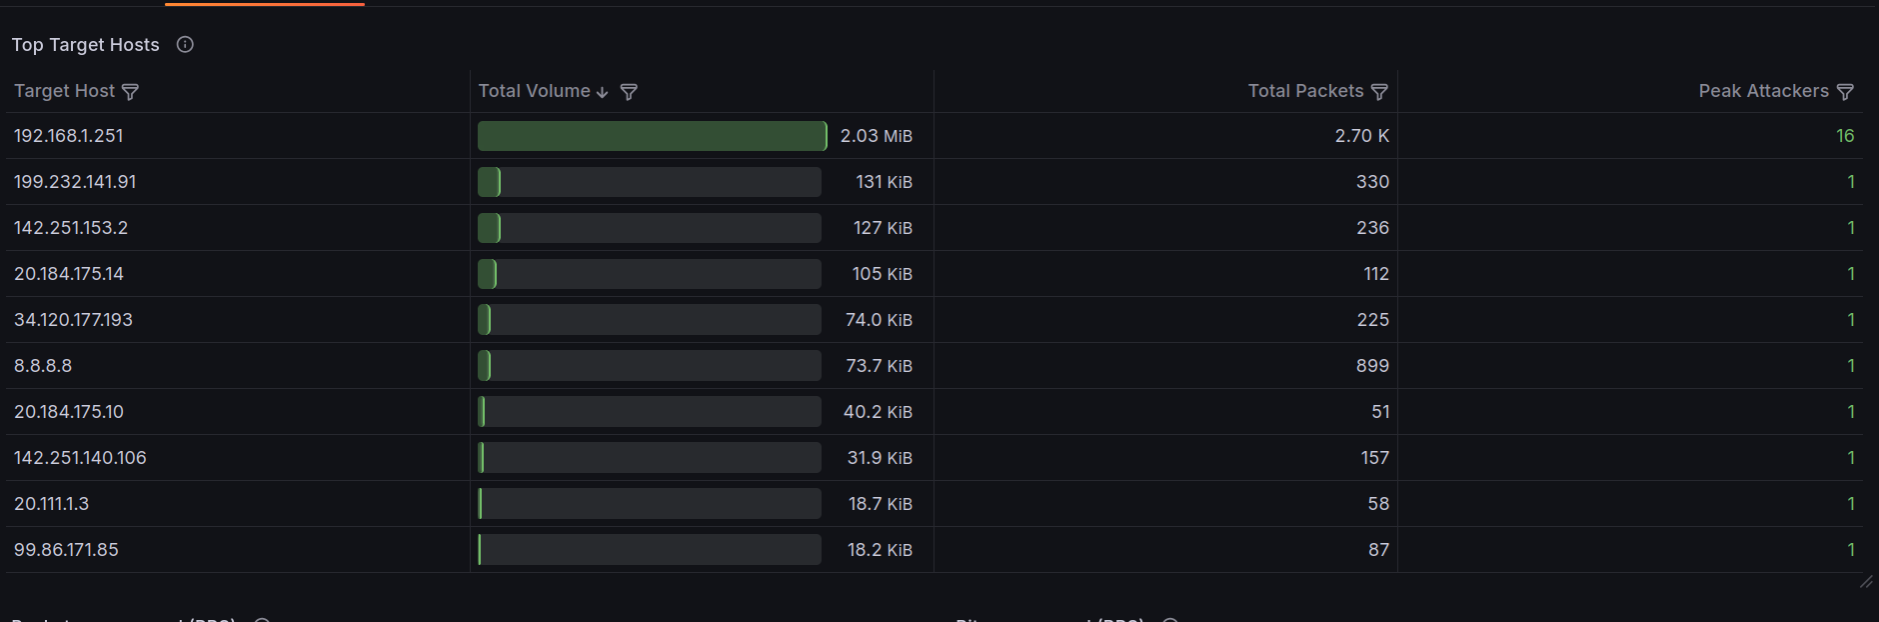
\includegraphics[width=0.95\textwidth]{it_p1.png}
    \caption{Inbound Traffic --- Top Target Hosts.}
    \label{fig:it_p1}
\end{figure}

\begin{figure}[htbp]
    \centering
    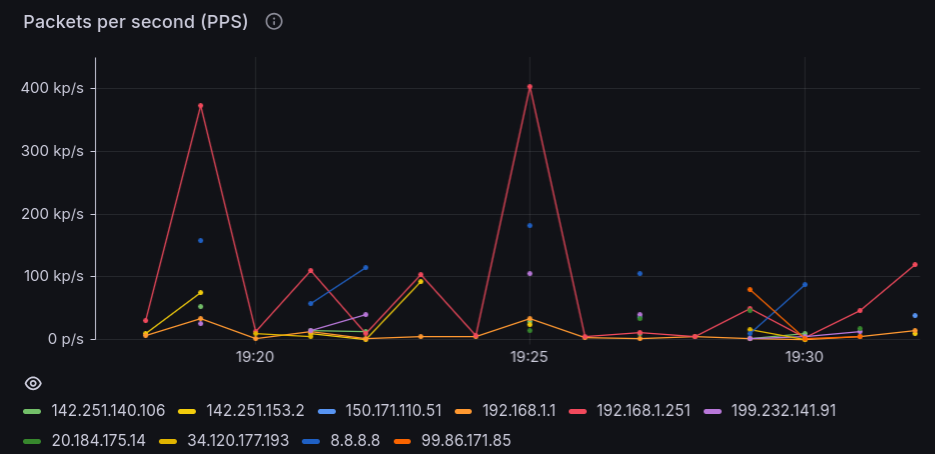
\includegraphics[width=0.95\textwidth]{it_p2.png}
    \caption{Inbound Traffic --- Inbound Packets per Second (PPS).}
    \label{fig:it_p2}
\end{figure}

\begin{figure}[htbp]
    \centering
    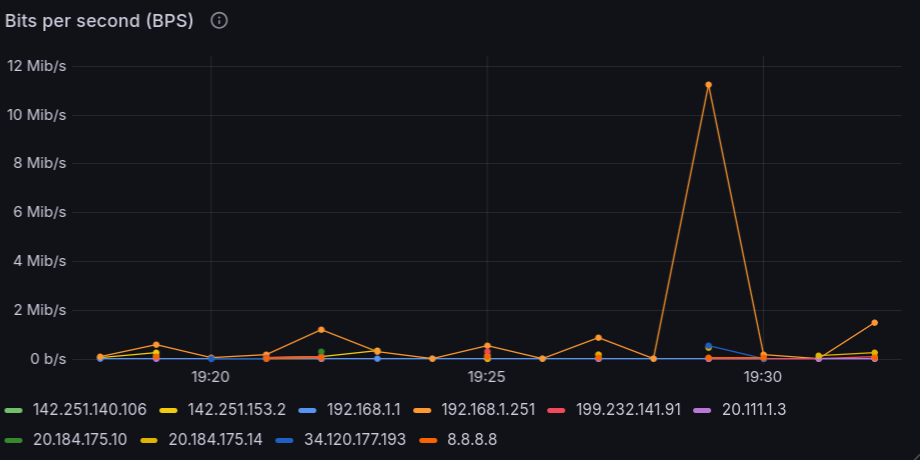
\includegraphics[width=0.95\textwidth]{it_p3.png}
    \caption{Inbound Traffic --- Inbound Bits per Second (BPS).}
    \label{fig:it_p3}
\end{figure}
\FloatBarrier

\paragraph{2. Outbound Traffic}
Queries \texttt{chiba.host\_src\_view} to identify local top talkers. It correlates emitted traffic volumes with destination IP cardinality (\texttt{max(UNIQUE\_DSTADDR)}) and contacted destination port cardinality (\texttt{max(UNIQUE\_DSTPORT)}), tracking outbound bandwidth and packet rates over time (Figures~\ref{fig:ot_p1}--\ref{fig:ot_p3}).

\begin{figure}[htbp]
    \centering
    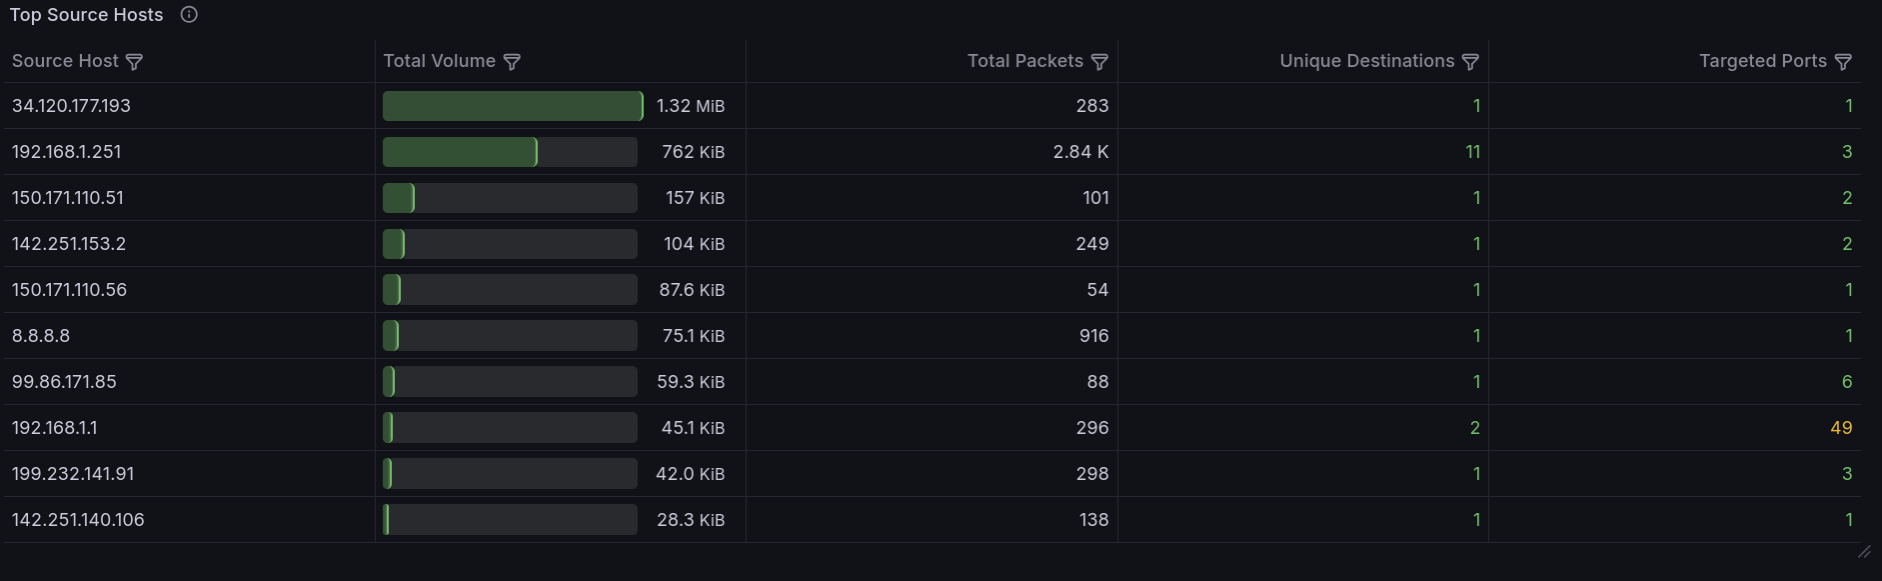
\includegraphics[width=0.95\textwidth]{ot_p1.png}
    \caption{Outbound Traffic --- Top Source Hosts.}
    \label{fig:ot_p1}
\end{figure}

\begin{figure}[htbp]
    \centering
    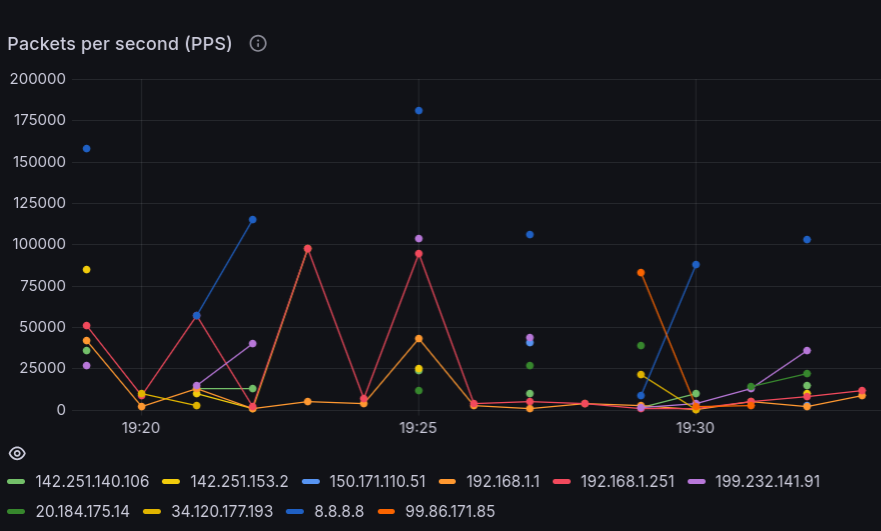
\includegraphics[width=0.95\textwidth]{ot_p2.png}
    \caption{Outbound Traffic --- Outbound Packets per Second (PPS).}
    \label{fig:ot_p2}
\end{figure}

\begin{figure}[htbp]
    \centering
    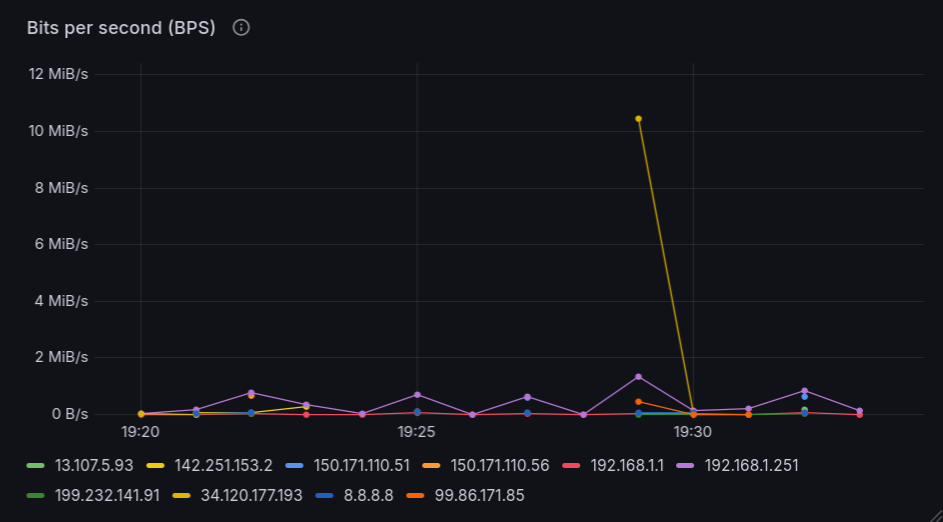
\includegraphics[width=0.95\textwidth]{ot_p3.png}
    \caption{Outbound Traffic --- Outbound Bits per Second (BPS).}
    \label{fig:ot_p3}
\end{figure}
\FloatBarrier

\paragraph{3. Protocol Distribution}
Relies on \texttt{chiba.service\_view} to segment traffic at Layer~4 and the application layer. It displays the percentage share of protocols (TCP, UDP, ICMP/ICMPv6), dominant destination services/ports, and protocol volume persistence over time (Figures~\ref{fig:pd_p1}--\ref{fig:pd_p3}).

\begin{figure}[htbp]
    \centering
    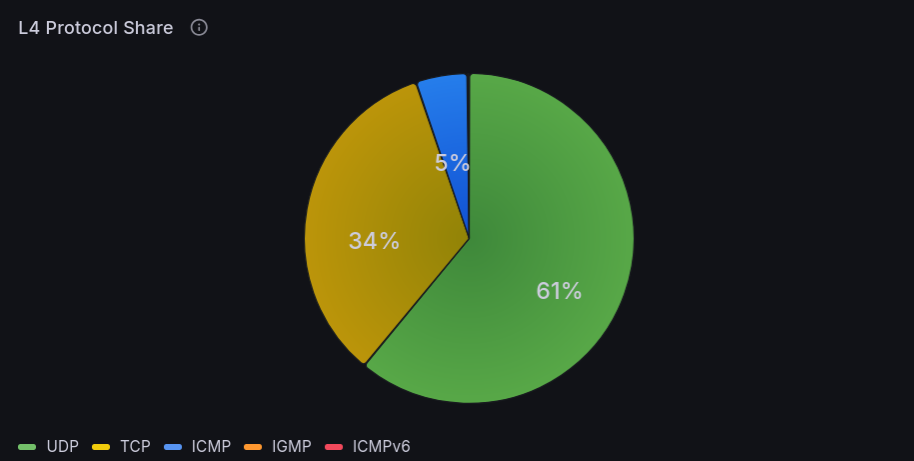
\includegraphics[width=0.95\textwidth]{pd_p1.png}
    \caption{Protocol Distribution --- L4 Protocol Share.}
    \label{fig:pd_p1}
\end{figure}

\begin{figure}[htbp]
    \centering
    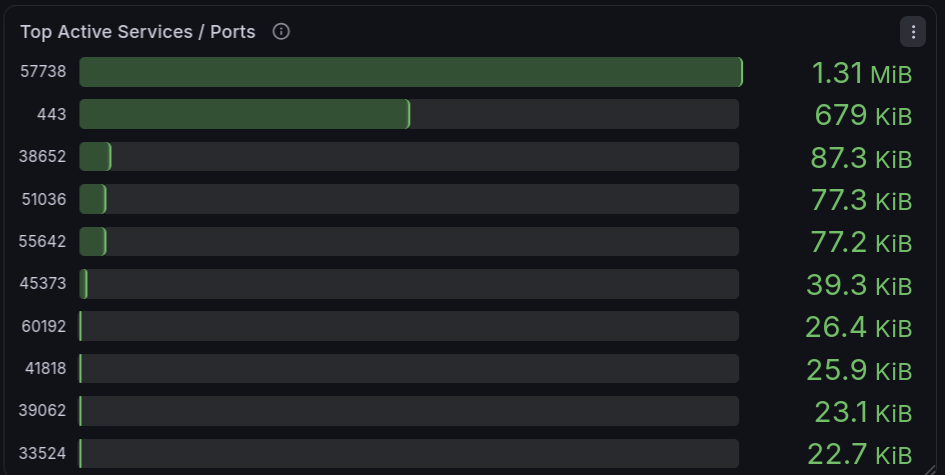
\includegraphics[width=0.95\textwidth]{pd_p2.png}
    \caption{Protocol Distribution --- Top Active Services / Ports.}
    \label{fig:pd_p2}
\end{figure}

\begin{figure}[htbp]
    \centering
    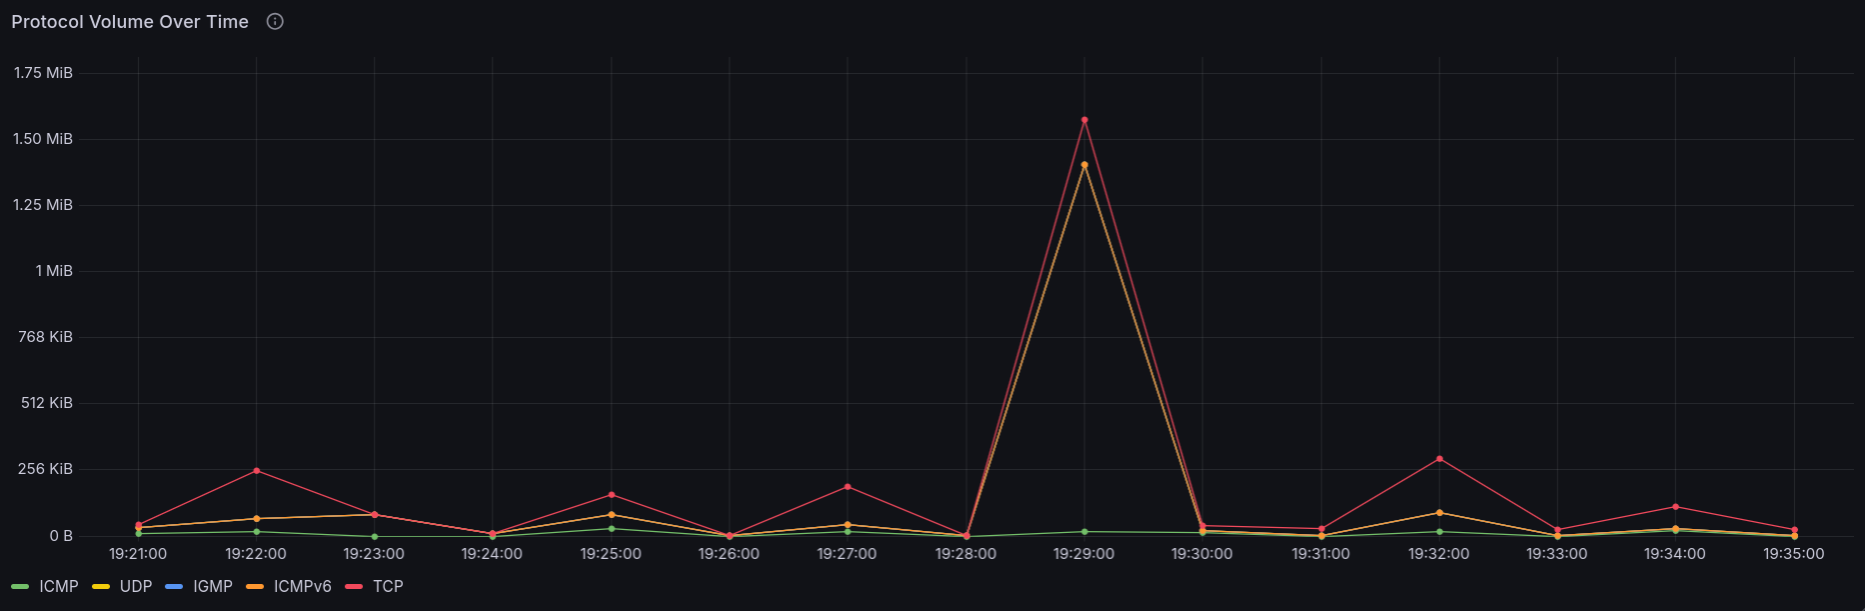
\includegraphics[width=0.95\textwidth]{pd_p3.png}
    \caption{Protocol Distribution --- Protocol Volume Over Time.}
    \label{fig:pd_p3}
\end{figure}
\FloatBarrier

\paragraph{4. Security Alerts}
Integrates four real-time status stat panels for immediate counting of hosts involved in malicious activity (DDoS targets, network scanners, port scanners, and high egress anomalies) and two detailed inspection tables for short-term (1-minute) and long-term (24-hour) security incidents (Figures~\ref{fig:sa_p1}--\ref{fig:sa_p3}).

\begin{figure}[htbp]
    \centering
    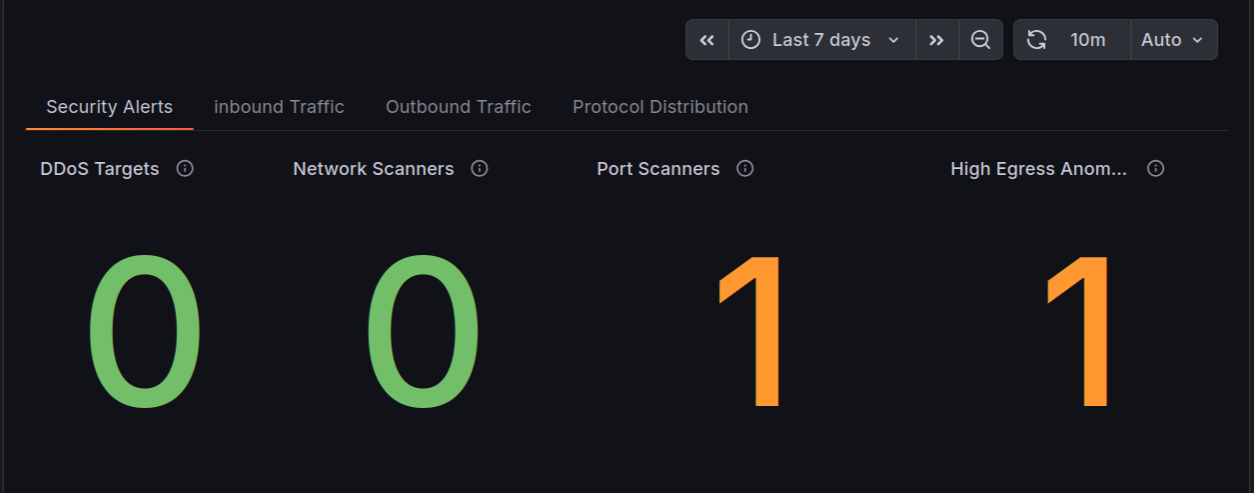
\includegraphics[width=0.95\textwidth]{sa_p1.png}
    \caption{Security Alerts --- Real-Time Threat Counters.}
    \label{fig:sa_p1}
\end{figure}

\begin{figure}[htbp]
    \centering
    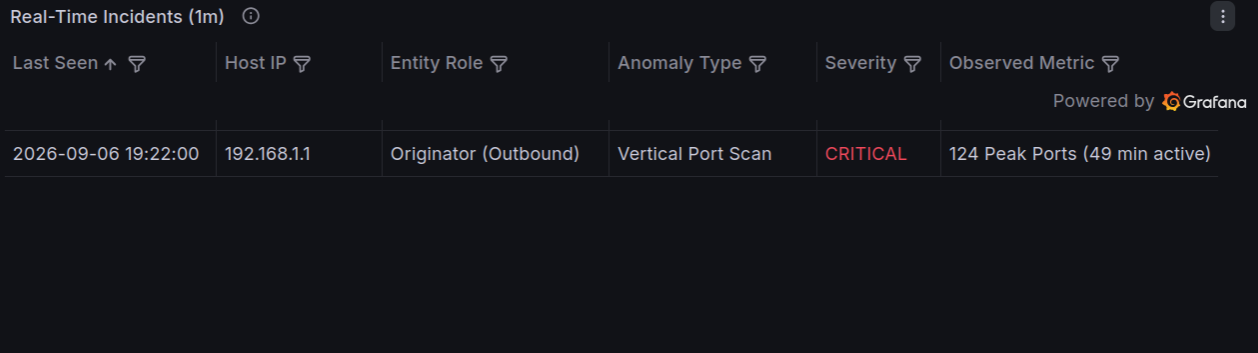
\includegraphics[width=0.95\textwidth]{sa_p2.png}
    \caption{Security Alerts --- Real-Time Incidents Table (1-Minute Window).}
    \label{fig:sa_p2}
\end{figure}

\begin{figure}[htbp]
    \centering
    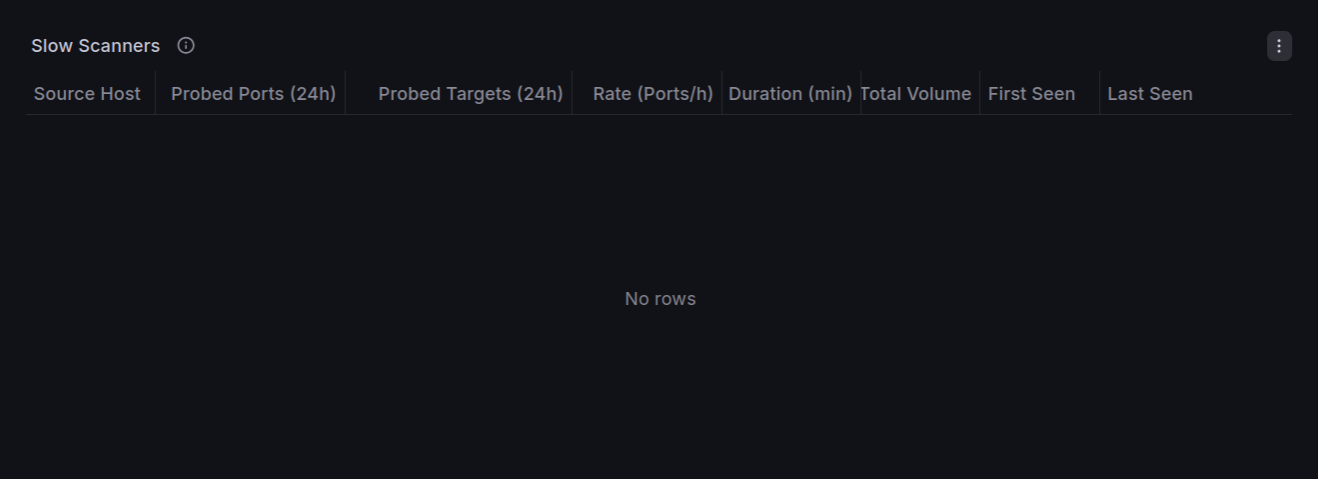
\includegraphics[width=0.95\textwidth]{sa_p3.png}
    \caption{Security Alerts --- Slow Scanners Table (24-Hour Sliding Window).}
    \label{fig:sa_p3}
\end{figure}
\FloatBarrier

\subsubsection{Detection Rules, Thresholds, and Severity}
The alerting engine separates the identification of rapid, volumetric anomalies over a 1-minute window from the analysis of slow, distributed reconnaissance anomalies over a 24-hour window.

The numerical thresholds adopted represent a heuristic baseline designed to enable reproducible laboratory testing, without claiming to mirror the exact traffic volumes of a large production network. Thanks to the strict architectural decoupling between the C capture daemon and the analytical layer, all detection logic resides exclusively inside Grafana queries and ClickHouse logical views: any threshold can therefore be recalibrated at runtime without altering the database schema or recompiling the C daemon.

\paragraph{1. Real-Time Detection (Window: 1 Minute)}
High-frequency anomalies are detected by aggregating \texttt{host\_dst\_view} and \texttt{host\_src\_view} per 1-minute \texttt{TIME\_BUCKET}. Results are merged into a unified incident table via \texttt{UNION ALL}, assigning each event a host role, threat category, and dynamic severity level evaluated through ClickHouse's \texttt{multiIf()} function:
\begin{itemize}
    \item \textbf{Distributed Flood / DDoS (Inbound):} Triggered when \texttt{UNIQUE\_SRCADDR >= 50} toward a single \texttt{DSTADDR}. Severity is graded via \texttt{multiIf(max(UNIQUE\_SRCADDR) >= 200, 'CRITICAL', 'WARNING')}. The convergence of flows from dozens or hundreds of distinct sources within the same minute onto a single target node highlights a distributed volumetric attack (such as a SYN/UDP flood or botnet).
    \item \textbf{Horizontal Network Sweep (Outbound):} Detects local hosts with \texttt{UNIQUE\_DSTADDR >= 50}, escalating to \texttt{CRITICAL} when \texttt{max(UNIQUE\_DSTADDR) >= 200}. Contacting an anomalous number of distinct destination hosts within 60 seconds identifies horizontal subnet reconnaissance.
    \item \textbf{Vertical Port Scan (Outbound):} Detects source hosts with \texttt{UNIQUE\_DSTPORT >= 20}, escalating to \texttt{CRITICAL} when \texttt{max(UNIQUE\_DSTPORT) >= 100}. Dispersion across dozens or hundreds of target ports within a single minute isolates vertical port scanning aimed at mapping active services.
    \item \textbf{Excessive Outbound Volume (Outbound):} Monitors flows with \texttt{TOTAL\_DOCTETS >= 20971520} (20~MiB/min), assigning \texttt{CRITICAL} severity starting at \texttt{52428800} (50~MiB/min). This rule detects anomalous outbound traffic spikes caused by unauthorized bulk data exfiltration or compromised nodes participating in outbound attacks.
\end{itemize}
In all cases, the query quantifies incident persistence via \texttt{count()}, returning the number of 1-minute buckets in which the anomaly remained active during the selected time window.

\paragraph{2. Extended-Horizon Detection (Window: 24 Hours)}
Advanced port scanners and stealth reconnaissance tools (such as \texttt{nmap} using slow timing templates or the \texttt{-{}-scan-delay} flag) deliberately space out probes over time to stay below per-minute thresholds (\texttt{UNIQUE\_DSTPORT < 20}) and evade real-time detection.

To catch these patterns, the \emph{Slow Scanners} table queries \texttt{slow\_scanners\_view}, which aggregates 1-minute buckets over a rolling 24-hour window (\texttt{WHERE TIME\_BUCKET >= now() - INTERVAL 24 HOUR}) and applies a joint volume-and-persistence filter:

\begin{codebox}[title={24-Hour Stealth Scanner Filter (\texttt{sql/05\_views.sql})}]
\footnotesize
\begin{verbatim}
WHERE TIME_BUCKET >= now() - INTERVAL 24 HOUR
GROUP BY SRCADDR
HAVING (UNIQUE_DSTPORT >= 50 OR UNIQUE_DSTADDR >= 100)
   AND ACTIVE_SPAN_MINUTES >= 30
\end{verbatim}
\end{codebox}

\begin{itemize}
    \item \textbf{24-Hour Sliding Window:} The clause \texttt{WHERE TIME\_BUCKET >= now() - INTERVAL 24 HOUR} merges partial HyperLogLog and min/max states across the entire day, uncovering probes spaced several minutes or hours apart.
    \item \textbf{Temporal Persistence (\texttt{ACTIVE\_SPAN\_MINUTES >= 30}):} Computed via \texttt{dateDiff('minute', toDateTime(EXACT\_START), toDateTime(EXACT\_END))}, isolating sustained reconnaissance while filtering out isolated short bursts or transient false positives.
    \item \textbf{Normalized Scan Rate (\texttt{PORTS\_PER\_HOUR}):} Computed as \texttt{round(UNIQUE\_DSTPORT / greatest(1, (EXACT\_END - EXACT\_START) / 3600), 2)}. Using \texttt{greatest(1, ...)} prevents division by zero for activities lasting less than an hour, normalizing probe frequency on an hourly basis to estimate the probing rate of the offending host.
\end{itemize}

% =============================================================================
% SECTION 2: PREREQUISITES AND EXECUTION INSTRUCTIONS
% =============================================================================
\section{Prerequisites and Execution Instructions}

\subsection{System Requirements and Dependency Installation}
The software architecture relies on four core components: the C daemon (\texttt{chiba}), \texttt{softflowd}, ClickHouse, and Grafana. The following installation instructions refer to Debian/Ubuntu-based distributions.

\subsubsection{Development Toolchain, Libraries, and Capture Probe}
To compile the daemon and enable NetFlow capture and decoding, install the C build toolchain, \texttt{libcurl} development headers, and \texttt{softflowd}:
\begin{codebox}[title={Toolchain and Probe Installation}]
\footnotesize
\begin{verbatim}
sudo apt update
sudo apt install build-essential gcc make libcurl4-openssl-dev softflowd
\end{verbatim}
\end{codebox}

\subsubsection{ClickHouse Installation (Server and Client)}
ClickHouse can be installed using the official installation script, which sets up the binaries and registers the \texttt{systemd} service:
\begin{codebox}[title={ClickHouse Server \& Client Installation}]
\footnotesize
\begin{verbatim}
# Download and run the official ClickHouse installer
curl https://clickhouse.com/ | sh
sudo ./clickhouse install

# Start the service for the current session
sudo systemctl start clickhouse-server

# (Optional) Enable automatic startup at boot:
# sudo systemctl enable clickhouse-server

# Verify service status and installed version
clickhouse-client --query "SELECT version();"
\end{verbatim}
\end{codebox}

\subsubsection{Grafana and ClickHouse Plugin Installation}
\begin{codebox}[title={Grafana OSS and ClickHouse Datasource Plugin Installation}]
\footnotesize
\begin{verbatim}
# Configure official APT repository and install Grafana OSS
sudo apt install apt-transport-https software-properties-common wget
sudo mkdir -p /etc/apt/keyrings/
wget -q -O - https://apt.grafana.com/gpg.key | gpg --dearmor \
  | sudo tee /etc/apt/keyrings/grafana.gpg > /dev/null
echo "deb [signed-by=/etc/apt/keyrings/grafana.gpg] https://apt.grafana.com stable main" \
  | sudo tee /etc/apt/sources.list.d/grafana.list
sudo apt update && sudo apt install -y grafana

# Install the official ClickHouse datasource plugin for Grafana
sudo grafana-cli plugins install grafana-clickhouse-datasource

# Start the Grafana server daemon
sudo systemctl start grafana-server

# (Optional) Enable at boot:
# sudo systemctl enable grafana-server
\end{verbatim}
\end{codebox}

\subsubsection{Test Traffic Generation Tools}
To run the security validation tests and traffic simulations described in Section~3:
\begin{codebox}[title={Traffic Simulation Utilities}]
\footnotesize
\begin{verbatim}
sudo apt install nmap hping3 netcat-openbsd tcpreplay
\end{verbatim}
\end{codebox}

\subsection{Compiling the CHIBA Daemon}
Building the executable is automated by the \texttt{Makefile} in the project root. Running \texttt{make} compiles all source modules in \texttt{src/}, creates the intermediate object directory \texttt{build/}, and produces the compiled binary at \texttt{bin/chiba}:
\begin{codebox}[title={Compiling and Cleaning}]
\footnotesize
\begin{verbatim}
# Compile the daemon
make

# Remove object files and compiled binaries
make clean
\end{verbatim}
\end{codebox}

\subsection{Database Initialization and Management}
The \texttt{Makefile} includes dedicated targets to sequentially execute all SQL schema scripts located in \texttt{sql/} (\texttt{00\_init.sql} $\rightarrow$ \texttt{05\_views.sql}), provisioning the \texttt{chiba} database, base table, intermediate state tables, materialized views, and logical views:
\begin{codebox}[title={Database Schema Management}]
\footnotesize
\begin{verbatim}
# Initialize the full database schema:
make db-init

# Full database reset (Drop and Re-init):
# Useful during testing to clear all table states.
# Prompts for explicit confirmation ('yes') to prevent accidental data loss:
make db-reset
\end{verbatim}
\end{codebox}

\subsection{Daemon Configuration and Execution}
HTTP connection parameters for ClickHouse are defined in \texttt{chiba.conf} in the project root:
\begin{codebox}[title={\texttt{chiba.conf}}]
\footnotesize
\begin{verbatim}
CH_HOST=http://127.0.0.1:8123
CH_DB=chiba
CH_TABLE=ingest_flows
\end{verbatim}
\end{codebox}
These parameters can be overridden at runtime using environment variables of the same name (\texttt{CH\_HOST}, \texttt{CH\_DB}, \texttt{CH\_TABLE}).

As described in Section~1.2, the daemon supports two mutually exclusive execution modes:
\begin{codebox}[title={Running CHIBA}]
\footnotesize
\begin{verbatim}
# Live capture on a network interface
# (requires root privileges for raw sockets in softflowd)
sudo ./bin/chiba -i <network interface name>

# Offline analysis of a static PCAP file
./bin/chiba -r ./pcap/DHCPv6.pcap
\end{verbatim}
\end{codebox}

\subsection{Grafana Dashboard Configuration}
\begin{enumerate}
    \item Open the Grafana web interface at \texttt{http://localhost:3000} (default credentials: username \texttt{admin}, password \texttt{admin}).
    \item From the side menu, navigate to \textbf{Connections} $\rightarrow$ \textbf{Data sources} $\rightarrow$ \textbf{Add data source} and select \textbf{ClickHouse}:
    \begin{itemize}
        \item \textbf{Server address:} \texttt{127.0.0.1}
        \item \textbf{Server port:} \texttt{8123}
        \item \textbf{Default database:} \texttt{chiba}
        \item Click \textbf{Save \& test} to verify connectivity with the DBMS.
    \end{itemize}
    \item Navigate to \textbf{Dashboards} $\rightarrow$ \textbf{New} $\rightarrow$ \textbf{Import}, click \textbf{Upload dashboard JSON file}, and select \texttt{grafana/chiba\_dashboard.json}.
\end{enumerate}

% =============================================================================
% SECTION 3: TESTING
% =============================================================================
\section{Testing}

\subsection{Fast Port Scan}
The objective of this test is to verify the detection of an aggressive vertical port scan against a single target host, exceeding the alarm threshold of 20 distinct destination ports within a 1-minute bucket.

The command used to generate the anomaly on the loopback interface is:
\begin{codebox}[title={Fast Vertical Port Scan Simulation}]
\footnotesize
\begin{verbatim}
sudo nmap -sS -T4 -p 1-150 127.0.0.1
\end{verbatim}
\end{codebox}

After the flow flush interval (60 seconds), querying \texttt{chiba.host\_src\_view} directly confirms proper flow aggregation:
\begin{codebox}[title={ClickHouse Verification Query}]
\footnotesize
\begin{verbatim}
clickhouse-client --query "
SELECT
    SRCADDR,
    UNIQUE_DSTPORT,
    PROT
FROM chiba.host_src_view
WHERE UNIQUE_DSTPORT >= 20;
"
\end{verbatim}
\end{codebox}

Output:
\begin{codebox}
\footnotesize
\begin{verbatim}
::ffff:127.0.0.1    150    6
\end{verbatim}
\end{codebox}

In the Grafana dashboard, the incident is immediately reflected in the alerting panels:
\begin{itemize}
    \item The \textbf{Port Scanners} counter increments to \texttt{1}.
    \item \textbf{Real-Time Incidents (1m) Table:} Host \texttt{127.0.0.1} is logged with anomaly type \texttt{Vertical Port Scan} and severity \texttt{CRITICAL} (having exceeded 100 ports).
\end{itemize}

\subsection{Network Sweep (Horizontal Scan)}
The objective of this test is to verify the detection of horizontal subnet reconnaissance aimed at mapping active hosts, exceeding the alarm threshold of 50 distinct destination addresses within 1 minute.

On Linux, the entire \texttt{127.0.0.0/8} subnet responds on the loopback interface. The command used to generate TCP probes toward 65 distinct IP addresses is:
\begin{codebox}[title={Horizontal Network Sweep Simulation}]
\footnotesize
\begin{verbatim}
sudo nmap -sS -T4 -p 80 127.0.0.1-65
\end{verbatim}
\end{codebox}

At the end of the aggregation interval, querying \texttt{chiba.host\_src\_view} confirms that the threshold has been exceeded:
\begin{codebox}[title={ClickHouse Verification Query}]
\footnotesize
\begin{verbatim}
clickhouse-client --query "
SELECT
    SRCADDR,
    UNIQUE_DSTADDR,
    PROT
FROM chiba.host_src_view
WHERE UNIQUE_DSTADDR >= 50;
"
\end{verbatim}
\end{codebox}

Output:
\begin{codebox}
\footnotesize
\begin{verbatim}
::ffff:127.0.0.1    65    6
\end{verbatim}
\end{codebox}

In the dashboard, the event is promptly displayed in the Security Alerts row:
\begin{itemize}
    \item The \textbf{Network Scanners} counter increments to \texttt{1}.
    \item \textbf{Real-Time Incidents (1m) Table:} Host \texttt{127.0.0.1} is reported with role \texttt{Originator (Outbound)}, anomaly \texttt{Horizontal Network Sweep}, and severity \texttt{WARNING} (severity escalates to \texttt{CRITICAL} above 200 destinations).
\end{itemize}

\subsection{Distributed Flood / DDoS}
The objective of this test is to verify the system's ability to intercept converging volumetric attacks, detecting when a single target host receives traffic from at least 50 distinct source IPs within 60 seconds.

The command uses \texttt{hping3} to transmit 80 TCP SYN packets toward the loopback address using spoofed random source IP addresses via the \texttt{-{}-rand-source} flag:
\begin{codebox}[title={Distributed SYN Flood Simulation}]
\footnotesize
\begin{verbatim}
sudo hping3 -c 80 -d 10 -S -p 80 --rand-source 127.0.0.1
\end{verbatim}
\end{codebox}

Querying \texttt{chiba.host\_dst\_view} highlights the concentration of concurrent sources on the target:
\begin{codebox}[title={ClickHouse Verification Query}]
\footnotesize
\begin{verbatim}
clickhouse-client --query "
SELECT
    DSTADDR,
    UNIQUE_SRCADDR
FROM chiba.host_dst_view
WHERE UNIQUE_SRCADDR >= 50;
"
\end{verbatim}
\end{codebox}

Output:
\begin{codebox}
\footnotesize
\begin{verbatim}
::ffff:127.0.0.1    80
\end{verbatim}
\end{codebox}

The incident is immediately reflected in the monitoring panels:
\begin{itemize}
    \item The \textbf{DDoS Targets} counter increments to \texttt{1}.
    \item \textbf{Real-Time Incidents (1m) Table:} Target \texttt{127.0.0.1} is recorded with role \texttt{Target (Inbound)}, anomaly \texttt{Distributed Flood}, and severity \texttt{WARNING}.
\end{itemize}

\subsection{Anomalous Egress Volume (Data Exfiltration)}
The objective of this test is to verify alerting on anomalous outbound traffic flows exceeding the volumetric threshold of 20~MiB (20,971,520 bytes) within 1 minute.

The test spawns a local listener on port 9999 and transfers 30~MiB of random data over loopback using \texttt{dd} and \texttt{nc}:
\begin{codebox}[title={Bulk Egress Transfer Simulation}]
\footnotesize
\begin{verbatim}
# Start local listener in background
nc -l -p 9999 > /dev/null &

# Bulk transfer of 30 MiB
dd if=/dev/urandom bs=1M count=30 | nc -w 1 127.0.0.1 9999
\end{verbatim}
\end{codebox}

Querying \texttt{chiba.host\_src\_view} confirms accurate quantification of the emitted byte volume:
\begin{codebox}[title={ClickHouse Verification Query}]
\footnotesize
\begin{verbatim}
clickhouse-client --query "
SELECT
    SRCADDR,
    formatReadableSize(TOTAL_DOCTETS) AS volume,
    TOTAL_DOCTETS
FROM chiba.host_src_view
WHERE TOTAL_DOCTETS >= 20971520;
"
\end{verbatim}
\end{codebox}

Output:
\begin{codebox}
\footnotesize
\begin{verbatim}
::ffff:127.0.0.1    30.00 MiB    31457280
\end{verbatim}
\end{codebox}

In the dashboard, the volumetric anomaly is displayed with automatic unit formatting:
\begin{itemize}
    \item The \textbf{High Egress Anomalies} counter increments to \texttt{1}.
    \item \textbf{Real-Time Incidents (1m) Table:} A record is generated for host \texttt{127.0.0.1} with type \texttt{Excessive Outbound Volume} and severity \texttt{WARNING} (escalating to \texttt{CRITICAL} above 50~MiB).
\end{itemize}

\subsection{Dual-Stack IPv6 Support from PCAP Trace}
The objective of this test is to validate offline processing of static PCAP traces and demonstrate that the NetFlow v9 parser accurately handles native 128-bit IPv6 addresses without memory corruption or endianness misalignment.

The command launches the daemon in offline mode on the IPv6 test capture:
\begin{codebox}[title={Offline IPv6 PCAP Ingestion}]
\footnotesize
\begin{verbatim}
./bin/chiba -r ./pcap/DHCPv6.pcap
\end{verbatim}
\end{codebox}

In PCAP mode, flows are recorded with the current system timestamp (\texttt{time(NULL)}), making them immediately visible in the Grafana dashboard without having to adjust the time picker to historical dates.

Querying \texttt{chiba.ingest\_flows} verifies the presence of native IPv6 addresses lacking the IPv4-mapped prefix (\texttt{::ffff:}):
\begin{codebox}[title={ClickHouse Native IPv6 Verification Query}]
\footnotesize
\begin{verbatim}
clickhouse-client --query "
SELECT
    toDateTime(START_TIME) AS time,
    IPv6NumToString(SRCADDR) AS src,
    IPv6NumToString(DSTADDR) AS dst,
    SRCPORT,
    DSTPORT,
    PROT
FROM chiba.ingest_flows
WHERE notLike(IPv6NumToString(SRCADDR), '::ffff:%')
LIMIT 5;
"
\end{verbatim}
\end{codebox}

Output:
\begin{codebox}
\footnotesize
\begin{verbatim}
2026-09-20 16:50:00  fe80::a00:27ff:fed4:10bb  fe80::a00:27ff:fefe:8f95  547  546  17
2026-09-20 16:50:00  fe80::a00:27ff:fed4:10bb  ff02::16                  0    0    255
2026-09-20 16:50:00  fe80::a00:27ff:fed4:10bb  ff02::1:fffe:8f95         0    0    58
2026-09-20 16:50:00  fe80::a00:27ff:fefe:8f95  fe80::a00:27ff:fed4:10bb  0    0    58
2026-09-20 16:50:00  fe80::a00:27ff:fefe:8f95  ff02::1:2                 546  547  17
\end{verbatim}
\end{codebox}

In the \emph{Protocol Distribution} row, IPv6 flows are aggregated accurately:
\begin{itemize}
    \item The \textbf{L4 Protocol Share} pie chart properly separates UDP and ICMPv6 (protocol 58) traffic.
    \item The service volume table records DHCPv6 ports (\texttt{546} and \texttt{547}) and Neighbor Discovery messages.
\end{itemize}

\subsection{Slow Port Scan (24-Hour Window)}
The objective of this test is to demonstrate the effectiveness of the extended-horizon detection engine: a low-frequency stealth reconnaissance diluted over time evades per-minute checks but is caught by the 24-hour sliding window view.

A diluted scan (for example, executed via \texttt{nmap -T1} or by setting an explicit probe delay with \texttt{-{}-scan-delay 15s}) keeps the number of probes per individual minute consistently below the fast threshold (\texttt{UNIQUE\_DSTPORT < 20}).

While \texttt{host\_src\_view} raises no alerts for any single 1-minute bucket, querying the 24-hour view \texttt{slow\_scanners\_view} correlates the cumulative probes once persistence and cardinality criteria (\texttt{ACTIVE\_SPAN\_MINUTES >= 30} and \texttt{UNIQUE\_DSTPORT >= 50}) are met:
\begin{codebox}[title={ClickHouse 24-Hour Slow Scanner Verification Query}]
\footnotesize
\begin{verbatim}
clickhouse-client --query "
SELECT
    SRCADDR,
    UNIQUE_DSTPORT,
    ACTIVE_SPAN_MINUTES,
    PORTS_PER_HOUR
FROM chiba.slow_scanners_view;
"
\end{verbatim}
\end{codebox}

Output:
\begin{codebox}
\footnotesize
\begin{verbatim}
::ffff:127.0.0.1    60    35    102.86
\end{verbatim}
\end{codebox}

This dual-horizon behavior is clearly reflected in the dashboard:
\begin{itemize}
    \item \textbf{Real-Time Incidents (1m) Table:} Zero alerts generated for individual 60-second buckets (confirming successful evasion of real-time per-minute thresholds).
    \item \textbf{Slow Scanners (24h Window) Table:} The offending host is surfaced along with its normalized \texttt{Rate (Ports/h)} metric, exposing the stealth reconnaissance activity.
\end{itemize}

% =============================================================================
% SECTION 4: CONCLUSIONS AND FUTURE WORK
% =============================================================================
\section{Conclusions and Future Work}
We can now draw several conclusions regarding the project.

The architecture is built around a core principle: a network monitoring system must operate autonomously, without requiring manual intervention to aggregate data or correlate anomalies that can be identified algorithmically in software. For this reason, metric computation and anomalous host identification occur entirely automatically inside ClickHouse.

At the same time, to prevent alert fatigue from causing operators to overlook real threats, the system clearly separates statistical anomaly warnings (\texttt{WARNING}) from severe, high-confidence incidents (\texttt{CRITICAL}), and combines a short-term 1-minute detection window with a 24-hour sliding window---filtering out normal network fluctuations while surfacing slow, persistent scans. Finally, to ensure critical alerts never go unnoticed, security indicators are placed at the top visual hierarchy of the dashboard to immediately capture operator attention.

Below are several directions for future development:
\begin{itemize}
    \item \textbf{Docker Compose Orchestration:} Coordinate the deployment, networking, and provisioning of ClickHouse, Grafana, \texttt{softflowd}, and CHIBA through a single \texttt{docker-compose.yml} specification.
    \item \textbf{Structured Logging System in C:} Replace formatted terminal print statements with a level-based structured logging subsystem (\texttt{DEBUG}, \texttt{INFO}, \texttt{ERROR}), which will be especially valuable as the codebase grows.
    \item \textbf{External Alert Notifications:} Dispatch automated notifications via email, Telegram, Discord, or webhooks whenever \texttt{CRITICAL} incidents are triggered.
    \item \textbf{Dynamic Baseline Thresholds:} Complement static heuristic thresholds with statistical baselines computed over historical network traffic, continuously adapting anomaly boundaries to the monitored environment.
\end{itemize}

% =============================================================================
% SECTION 5: REFERENCES AND BIBLIOGRAPHY
% =============================================================================
\section{References and Bibliography}
\begin{itemize}
    \item Brian ``Beej Jorgensen'' Hall, \emph{Beej's Guide to Network Programming --- Using Internet Sockets}: \url{https://beej.us/guide/bgnet/html/}
    \item Michael Kerrisk, \emph{The Linux Programming Interface}: No Starch Press
    \item Luca Deri, \emph{Network Monitoring in Practice}: \url{https://luca.ntop.org/gr2026/tm2026.pdf}
    \item Cisco Systems, \emph{RFC 3954 --- Cisco Systems NetFlow Services Export Version 9}: \url{https://datatracker.ietf.org/doc/html/rfc3954}
    \item IANA (Internet Assigned Numbers Authority), \emph{Protocol Numbers}: \url{https://www.iana.org/assignments/protocol-numbers/protocol-numbers.xhtml}
    \item ClickHouse Official Documentation: \url{https://clickhouse.com/docs}
    \item Grafana Official Documentation: \url{https://grafana.com/docs}
\end{itemize}

\end{document}
